% %This is a very basic essay template based on letter class.
\documentclass[12pt,a4paper]{article}
\usepackage{ucs}
\usepackage[T2A]{fontenc} 
\usepackage[utf8]{inputenc}
\usepackage[english,bulgarian]{babel} 
\usepackage[margin=1in]{geometry}
% \usepackage[bindingoffset=2cm,centering,includeheadfoot,margin=1in]{geometry}
\usepackage{graphicx}
\usepackage{setspace}
\onehalfspacing


\begin{document}

\thispagestyle{empty}
\begin{titlepage}
\begin{center}
\newcommand{\HRule}{\rule{\linewidth}{0.5mm}}

% Upper part of the page
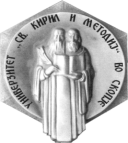
\includegraphics[width=0.15\textwidth]{images/ukim}\\[1cm]
\textsc{\large Универзитет „Св. Кирил и Методиј“ - Скопје}\\[1.5cm]


\includegraphics[width=0.3\textwidth]{images/finki_logo}\\[1cm]
\textsc{\large Факултет за информатички науки и компјутерско
инженерство}\\[1.5cm]

% Title
\HRule \\[0.4cm]
{  \bfseries \textsc{Зошто да изучуваме етика?} \\[0.4cm] - есеј
-}
\vfill
\emph{„Живеј како да ти е последен ден. Учи како кога би живеел вечно.“} - Ганди
\vfill
\\[0.4cm]

\HRule \\[1.5cm]

% Author and supervisor
\begin{minipage}{0.45\textwidth}
\begin{flushleft} 
\emph{Студент:}\\
М-р Томче \textsc{Делев}\\
tomche.delev@finki.ukim.mk
\end{flushleft}
\end{minipage}
\begin{minipage}{0.45\textwidth}
\begin{flushright} 
\emph{Ментор:} \\
Д-р Кирил \textsc{Темков}
\end{flushright}
\end{minipage}

\vfill

% Bottom of the page
{\large Мај 2012}

\end{center}
\end{titlepage}

Со успех и посветеност го завршив основното и средното образование. Дипломирав и
магистрирав на технички факултет и до овој момент кога сум дел од докторска
школа не сум имал можност или среќа да учествувам или бидам дел од некаква форма
на етичко образование. Денес слушам и читам за основните начела на етиката и
имам чувство како од секогаш да е всадено во мене знаење и размислувања за
најважните етички принципи и прашања. Секоја една одлука како да постапам во
одредена ситуација, како да се однесувам, да разликувам помеѓу добро и лошо,
всушност претставува етичко прашање. Што е тоа што е добро за мене, за моите
најблиски, за поширокото опкружување? Како да постапувам во животот, кои да
бидат моите цели и кој е патот по кој ќе ги остварувам? Во текот на целиот живот
се соочуваме со овие и безброј други етички прашања.

Можеби формално не сум ја изучувал етиката или моралните вредности, но животното
искуство од раѓањето, од првата самостојна одлука, од првиот контакт со
општеството е секојдневно практикување етика. Секојдневно се соочуваме со
ситуации во кои бараме и наоѓаме одговори на етички прашања? Но дали ги знаеме
вистинските одговори на овие прашања? Дали постојат вистински одговори? Од што
зависи како ќе се однесуваме и како ќе пристапиме кон овие прашања? Кои се
моралните принципи според кои ќе живееме?

Сакам да поставам и уште едно прашање? Дали треба да знаеме повеќе за основните
етички прашања и дали тоа ќе не направи подобри луѓе? И конечно, дали сите луѓе
имаат право да научат повеќе за најважните прашања во животот? Да дознаат повеќе
за прашањата чии одговори ја формираат нивната личност, за одлуките кои ќе им го
трасираат патот до целта\ldots

Човекот се раѓа и расте во контролирана заедница наречена семејство. Оваа микро
околина е неговиот прв контакт со светот. Во оваа околина новороденчето станува
дете, расте и се развива и се оформува во посебна индивидуа и ги учи одговорите
на првите прашања на животот. А какви се прашањата на животот ако не етички? Ова
е таа етика за која сите знаеме нешто и ја чуствуваме како вградена во нашата
ДНК. И таа некогаш сме ја научиле од некој, сме ја виделе некаде и сме ги
почуствувале последиците од неа. Тоа е етиката на нашите родители, на нашето
семејство и тоа во контекст на времето во кое живееме, културата и религијата во
која растеме и се развиваме.

Националноста, културата и религијата се многу значајни сегменти од животот и
нив детално и исцрпно ги разработува етиката. Сите заедно имаат големо значење
за етиката и моралните норми на кои се учиме. Но сепак неоспорен е фактот дека
семејството е една од најважните алки во моралното и етичкото оформување на
луѓето. Тоа е микросветот во кој тие осознаваат за светот, го имаат првиот допир
со реалноста и практично ги добиваат одговорите на првите етички прашања.
Семејството е етичкото образование на денешната генерација и многу генерации
наназад. За многу луѓе е сосема нормално една од улогите на семејството да биде
да ја создава етиката на своите членови. Но дали е ова секогаш добро? Дали ги
имаат сите семејстава истите морални вредности?

Најголем дел од децата имаат среќа да се раѓаат во оформени и нормални
семејства. Семејства кои го достигнале еден од основните стремежи на човекот да
го продолжува своето поколение и да расте и оформува нови здрави поколенија.
Семејства кои создаваат околина исполнета со луѓето кои не сакаат, кои се грижат
за нас и постојано се обидуваат да создадат добри личности, притоа следејќи ги
сопствените етички норми и принципи. Секое дете кое израснало како дел од здраво
и нормално семејство, одговорот на првите етички прашања го добива токму таму.
Тоа го слуша говорот на своите најблиски, го гледа и следи нивното однесување.
Семејството за детето е првата и најзначајна етичка библија.

Меѓутоа и во светот кој денес го знаеме, колку и да е променет и напреден, не
сите деца ја имаат среќата да растат во здрави и нормални семејства. Денес, како
никогаш порано сме сведоци на распаѓање на концептот на семејство во кој ние сме
растеле. Динамиката на животот и некои нови вредности создаваат сосема друга
околина во која многу „несреќни“ деца ќе треба да се оформуваат и учат за своите
први чекори во животот и општеството. Овде се наметнува уште едно многу важно и
суштинско прашање, дали овие деца заслужуваат подобро? Како овие нови и идни
носители на нашето општество ќе научат да се однесуваат добро, да имаат цел во
животот, да постигнуваат успех и на крај да бидат примерни и успешни граѓани?
Дали сите имаме подеднакво право да учиме и знаеме за вистинските етички
вредности? Дополнително, дали сите идни родители треба да учат како да се
однесуваат со своите деца и врз основа на кои етички принципи ќе го градат
семејството во кое ќе ги растат своите деца?

Одговорот на овие прашање го дава смислата на постоењето на етиката. Сите сакаме
свет во кој што ќе преовладува доброто однесување, ќе има високо ниво на култура
и разбирање. Знаењето и меѓусебното почитување очекуваме да биде највисока
вредност кај луѓето. Посакуваме да нема искривени вредности и моралот кај луѓето
да биде на највисоко ниво. Секој заслужува да ги осознае и научи за етичките
норми, за моралот и вистинските вредности и тоа во контекст на своето време.
Етиката колку и да е универзална, сепак треба да се пренесе на соодветен начин
прифатлив за општеството, во колосек со религијата и со сите останати сегменти
на живеењето во кои задира. Ова нималку не е лесно\ldots


Една од целите на изучувањето етика треба да биде да го трасира патот до многу
подобро општество во кое ќе сакаме да живееме и многу повеќе ќе се сакаме помеѓу
себе. Зошто по овој пат да не тргнеме со тоа што ќе изучуваме етика? Зошто да не
им се овозможи на децата уште од најмала возраст да слушаат и учат што е тоа што
е добро? Како да се биде добар? Кои се вистинските вредности и како да се бориме
за нив? Како да сакаме и да не ги повредуваме другите?

Историјата многу пати до сега била сведок дека цели империи, нации, општествени
уредувања се променети под влијание на некое учење и настојување да се
индоктринира одредена идеологија. Зошто таа доктрина да не биде учењето етика и
зошто не оставиме на времето да покаже за вистинските ефекти кои тоа ќе ги
постигне врз општеството, а кои сигурно нема да минат незабележано.

Без етичко образование всушност ние и никогаш не сме учеле етика. Ако ги
запрашате луѓето што не изучувале етика, дали знаат што е тоа етика, повеќето ќе
ви одговорат дека знаат. Но, ако ги запрашате што е тоа етика, повеќето ќе
одговорат нешто за кое претпоставуваат дека е етика или претставува етика.
Секогаш е добро да се има мислење за нешто, но многу е подобро е да се знае и
разбира тоа нешто, а секогаш е најдобро да се применува, па така и за етиката.
Можеби ќе дојде и тој ден кога вистинската етика ќе ја видиме и почуствуваме во
нашиот живот. И тоа да не биде како исклучок во општеството, туку како норма во
животот на мнозинството луѓе. Прочуениот кинески философ Конфучиј рекол
\emph{„Слушам, па заборавам. Гледам, па паметам. Правам, па разбирам.“} Да се
надеваме дека децата и возрасните што повеќе ќе слушаат за етика, ќе ја гледаат
околу себе и вистински ќе ја разбираат.


\end{document}
